\label{ch:sdr}

% Intro
While previous work utilized MOAA for delayed heating calculations \cite{fairhurst_decay_2022, fairhurst_demonstration_2022, fairhurst_database_2022}, a modification to the calculation workflow allows it to obtain the shutdown-dose rate.
The calculation workflow for the shutdown dose rate and delayed gamma heating is very similar, and they only change in how the deposition of energy manifests, either dose or heat.

% Motivation
The purpose of this chapter is to demonstrate the shutdown dose rate calculation workflow.
The development of experiment safety analysis also requires the determination of a \gls*{PIE} strategy, including the estimation of the dose rate in the surroundings of the experiments.
A capability like this allows to establish a \gls*{PIE} of an experiment from the dose rate standpoint, as well as design optimization.
% 
The equivalent dose rate from delayed gamma radiation is also an important factor for safely conducting work after reactor shutdown, such as periodic maintenance, fuel shuffling, among others \cite{ho_calculation_2022}.

Motivated by the calculation of shutdown dose rates in experiments, one experiment conducted at \gls*{ATR}, the \gls*{AGR1} \cite{sterbentz_agr1_2018}, requires special attention.
The \gls*{AGR1} was an experiment fueled with \gls*{TRISO} particles, which is a type of fuel form that is commonly found in \glspl*{HTGR}.
So, in order to properly model the AGR-1 experiment, it is insightful to understand the calculation workflow for shutdown dose rates in \glspl*{HTGR}.

% Shutdown dose rate in LWRs
Many publications have studied the shutdown dose rate in \glspl*{LWR}.
%
For example, Abrefah et al. \cite{abrefah_estimation_2018} estimated the dose rate of the spent fuel of the Ghana Research Reactor-1 (GHARR-1) to establish a proper unloading strategy for the \gls*{HEU} to \gls*{LEU} conversion of the reactor.
% The calculations used ORIGEN-S and MCNP6.
%
In another work, Ambrozic and Snoj \cite{ambrozic_JSIR2S_2020} studied the dose rate in the Jozef Stefan Institute (JSI) TRIGA reactor and validated their results against experimental measurements during normal operation and after shutdown.
% coupling MCNP6.2 and FISPACT-II
%
Bagheri et al. \cite{bagheri_gamma_2021} determined the dose rate from the spent fuel of the Tehran Research Reactor (TRR), validated their calculations against experimental measurements, and studied the photon emission rate of several isotopes for different fuel burnup values.
% Their calculations used ORIGEN2.1 and MCNPX2.7.

Although the shutdown dose rate associated with LWRs has been extensively studied, there are not many publicly available studies that focus on \glspl*{HTGR}.
%
For example, Suwoto et al. \cite{suwoto_neutron_2018} calculated the neutron dose rate in the working areas outside the \gls*{RPV} of the HTGR-10 reactor, concluding that the dose rates were compliant with the stipulated limits.
% MCNP5
% 
Ueta et al. \cite{ueta_shielding_2016} studied the shielding performance for the upper structure of the \gls*{HTTR} during normal operation.
Their study considered the active core, spent fuel, and equipment installed in the primary circuit as neutron and gamma radiation sources, and concluded that the neutron contribution to the dose was over 90\%.
% The spent fuel source was evaluated with ORIGEN2.
% 
Another study by Hamzah et al. \cite{hamzah_preliminary_2019} analyzed the dose rate distribution in the Reaktor Daya Eksperimental (RDE), a 10 MWth experimental pebble-bed reactor, during normal operation and after shutdown.
Their study estimated the dose rates in the working area and outside the RDE reactor building, concluding that the calculated values were below the stipulated limits.
% The latter relied on ORIGEN2 to determine the source strength of the decay gamma radiation.
%
% Conclusion
% Option 1
Ho et al. \cite{ho_calculation_2022} calculated the shutdown gamma distribution in the \gls*{HTTR}, relying on MCNP6 \cite{mcnp} and ORIGEN2 \cite{croff_origen2_1980} to obtain the gamma source distribution and MCNP6 to conduct the gamma transport at multiple cooling times.
Their work utilized the repeated structures from MCNP6 to model the decay sources from all the fuel rods explicitly, with the gamma radiation emitted from each rod with a uniform spatial distribution.
Most of the studies described above focus on the dose rates during normal operation or perform some level of homogenization to avoid the explicit modeling of the TRISO particles as decay radiation source.
% Option 2
% Up to this point, most of the studies described above focus mainly on the dose rates during normal operation or do not provide a thorough description of their methods for taking into account the decay gammas as a radiation source.
% % ho_calculation_2022
% In contrast, Ho et al. \cite{ho_calculation_2022} calculated the shutdown gamma distribution in the \gls*{HTTR} and provides a rigorous description of their implementation.
% Their calculations relied on MCNP6 \cite{mcnp} and ORIGEN2 \cite{croff_origen2_1980} to obtain the gamma source distribution and then their energy deposition was calculated using MCNP6 for different cooling times.
% Their work utilized the repeated structures from MCNP6 to model the sources from all the fuel rods explicitly with the gamma radiation emitted from each rod with a uniform spatial distribution.
% % Most of the studies focus mainly on the dose rates during normal operation or perform some sort of homogenization, neglecting the double heterogeneity of the fuel.

The objective of this work is to introduce a new shutdown dose rate calculation capability for TRISO-fueled experiments and HTGRs.
The modeling of HTGRs is challenging due to the fuel double heterogeneity, a distinctive characteristic in this type of reactor due to its fuel nature - i.e., the \gls*{TRISO} particles.
Previous work \cite{fairhurst_decay_2022, fairhurst_demonstration_2022, fairhurst_database_2022} utilized MOAA to calculate delayed heating by treating each depleted cell as an independent source of radiation.
However, one single HTGR core contains millions of TRISO particles, meaning that modeling each cell independently is not realistically possible.
This chapter of the thesis investigates the modeling of the AGR-1 experiment using the repeated structures from MCNP to explicitly model the TRISO particles as decay radiation source.

This chapter is organized as follows.
Section \ref{sec:methodology} details the main aspects of the calculation workflow.
Section \ref{sec:verif} introduces a verification exercise consisting of the delayed heating calculation of a simple geometry.
Section \ref{sec:agr} discusses an exercise studying the shutdown-dose rates of the \gls*{AGR1} experiment.
% \cite{fairhurst_sdr_2023}
Additionally, Section \ref{sec:micro} uses the workflow described here to study potential decommissioning strategies of a high-temperature gas-cooled microreactor.


\section{Methodology}
\label{sec:methodology}

% Intro: MOAA as the main solver
The calculations use the formal 3-step process to obtain the shutdown dose rates, consisting of the following three steps:
\begin{itemize}
  \item First, a neutron-transport simulation determines the neutron flux spatial and energy distribution during reactor operation.
  \item Second, an activation calculation estimates the energy distribution and emission probability of the decay photon sources after reactor shutdown.
  \item Third, a photon-transport simulation evaluates the dose rate.
\end{itemize}

% Workflow
As we can see, the calculation workflow for the shutdown dose rate and delayed gamma heating (Sec. \ref{sec:delheat}) is identical, and the only change is the evaluation of energy deposition resulting from the photon transport.
Overall, the calculation scheme, shown in Figure \ref{fig:workflow_4}, follows the formal 3-step process, in which MOAA conducts the first two steps, and an MCNP photon-transport simulation carries out the third step and estimates the dose rate with the following formula
% Photons deposit their energy globally thus requiring a transport simulation \cite{peterson-droogh_current_2018}.

% Formulas
% 1.6022 \times 10^{-19} \times 3600
\begin{align}
\dot{D}[Sv/h] &=  F4\!:\!p [pSv/src] \times \mathlarger{\sum}_i S_i \times 3.6 \times 10^{-9} \label{eq-dose} \\
S_i[\gamma/s] &= \int_{E} \varphi^\gamma_i(E) dE \\
s_i [-] &= S_i / \mathlarger{\sum}_j S_j
\end{align}
where $\dot{D}$ is the dose rate, $F4\!\!:\!\!p$ is the F4 tally for photons, $S_i$ is the total photon emission rate from region $i$, $\varphi^\gamma_i(E)$ is the photon source energy distribution from region $i$, and $s_i$ is the source emission probability of region $i$.
$F4\!\!:\!\!p$ result is expressed in $pSV$ per source particle by adding fluence-to-dose conversion factors \cite{icrp_116} to the MCNP input file.
The conversion factors consider an antero-posterior exposure to photons.

\begin{figure}[htbp!]
  \begin{center}
    
\includegraphics[width=0.85\linewidth]{figures/dose-flow}
  \end{center}
  \caption{Shutdown dose rate calculation scheme.}
  \label{fig:workflow_4}
\end{figure}


\section{Verification}
\label{sec:verif}

% Intro
This exercise consists of the delayed gamma heating calculation in a simple geometry.
The calculation workflow for the shutdown dose rate and delayed gamma heating is identical, and they only change in how the deposition of energy manifests, either dose or heat.
Three calculations were performed for this exercise.
The first calculation employs the explicit independent definition of each cell and provides the reference values.
The second calculation utilizes the repeated structures' approach.

The following equation calculates the delayed gamma heating
\begin{align}
H_{\gamma, Tr} [W] &= 1.6022 \times 10^{-13} \times \: ^* \! F8 [MeV] \times \mathlarger{\sum}_i S_i
\end{align}
where $H_{\gamma, Tr}$ is the energy deposited in the region of interest resulting from the photon transport, $^\ast F8$ is the energy deposition calculated by an $^\ast$F8 tally, and $S_i$ is the total photon emission rate from the region $i$ (see Eq. \ref{eq-ga-tr}).

% OLD RESULTS
% % Problem definition
% % Geometry
% The problem geometry is displayed in Figure \ref{fig:toy-geo2}.
% The core consists of a 4x4 array of fuel pins of 2.5 cm radius with an 8 cm pitch, and it is separated from the reflector tank by an inner shell of aluminum.
% The shell dimensions are an inner side length of 32 cm and a 2 cm thickness.
% The reflector tank is filled with light water, and its radius is 40 cm.
% The whole geometry has an 80 cm height.
% The fuel is 7.8\%-enriched uranium with a density of 10.5 g/cm$^3$, the inner shell is made of pure aluminum with a density of 2.7 g/cm$^3$, and the light water has a density of 1.0 g/cm$^3$.

% \begin{figure}[htbp!] %or H 
%     \centering
%     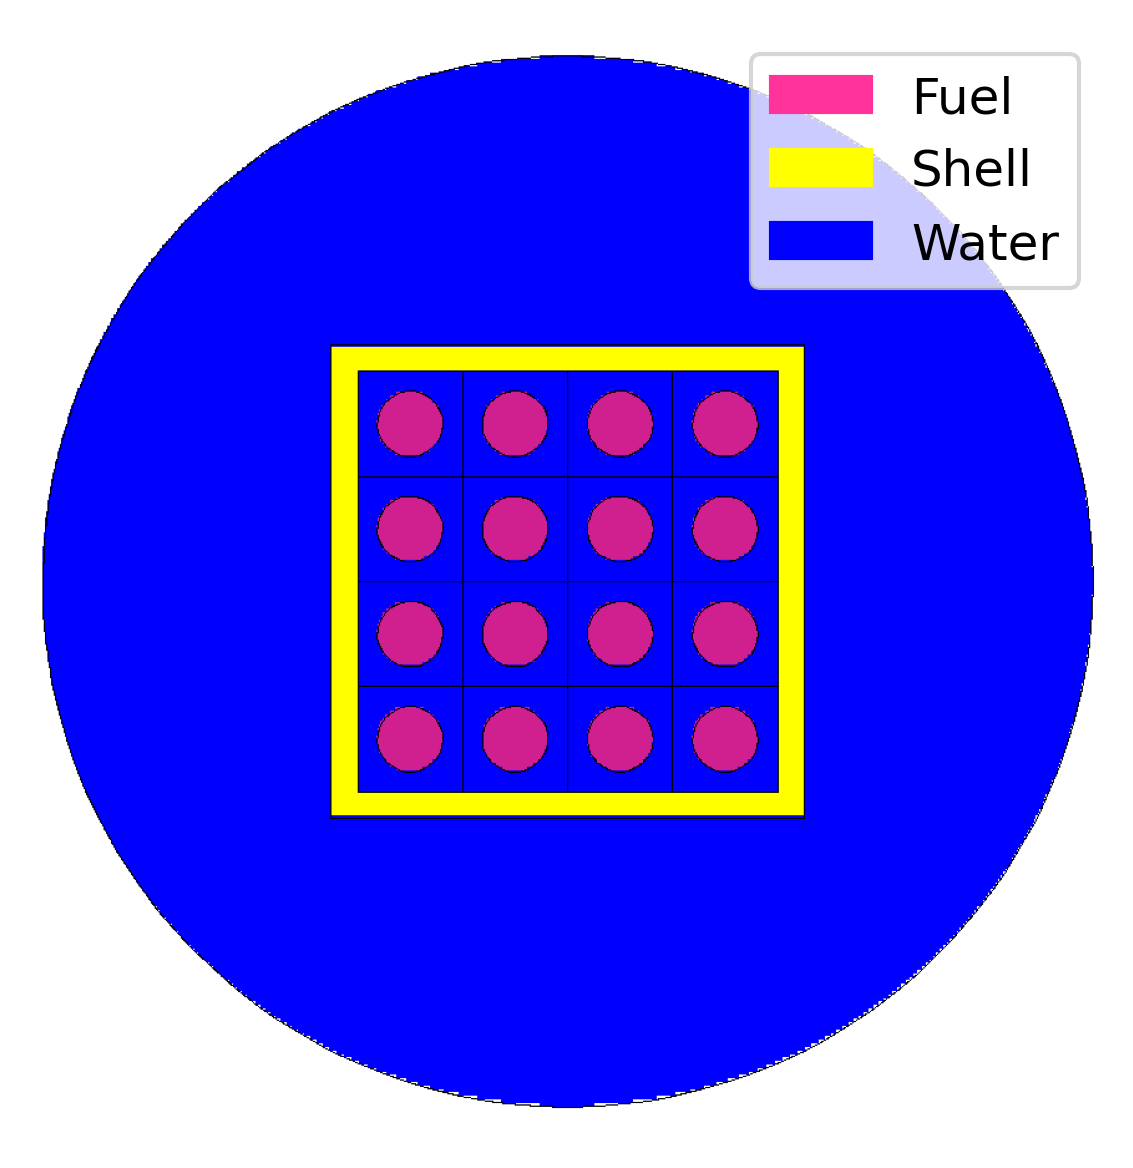
\includegraphics[width=0.60\linewidth]{figures/toy-problem.png}
%     \hfill
%     \caption{Verification problem geometry. The delayed gamma heating is calculated in the core inner shell.}
%     \label{fig:toy-geo2}
% \end{figure}

% % The Problem
% The main objective of the calculation is the estimation of the delayed gamma heating in the core inner shell, considering all the fuel pins as the radiation source.
% The delayed heating is calculated after a reactor operation at a 1 MW constant power for a 12-month cycle.

% % Results
% Table \ref{table:verif} summarizes the main results at the end of irradiation.
% While the heating equals 616.1 W in the reference case, the repeated structures' case predicts a heating of 685.2 W, which is 11.2\% larger than the reference value.
% To understand this result, we need to investigate other quantities in the results.
% The average neutron flux and total photon intensity show a relative difference smaller than 0.1\%.
% Figure \ref{fig:ver-comp} displays the uranium composition evolution during irradiation.
% The uranium evolution displays a relative difference smaller than 0.1\%.

% \begin{table}[!htb]
%   \centering
%   \caption{End of irradiation integral results.}
%   \label{table:verif} 
%   \begin{tabular}{l|cc|c}
%   \toprule
%           & Reference & Rep. Struct. & Rel. Diff. [\%] \\ % (RS/REF - 1)*100
%   \midrule
%    Delayed gamma heating [W]           &  616.1  &  685.2  & 11.2 \\
%    Ave. neutron flux [10$^{13}$ n/cm2/s] &  2.377  &  2.375  & 0.08 \\
%    Tot. photon intensity [10$^{17}$ $\gamma$/s] &  3.672  &  3.672  & 0.01 \\
%   \bottomrule
%   \end{tabular}
% \end{table}

% \begin{figure}[htbp!] %or H 
%     \centering
%     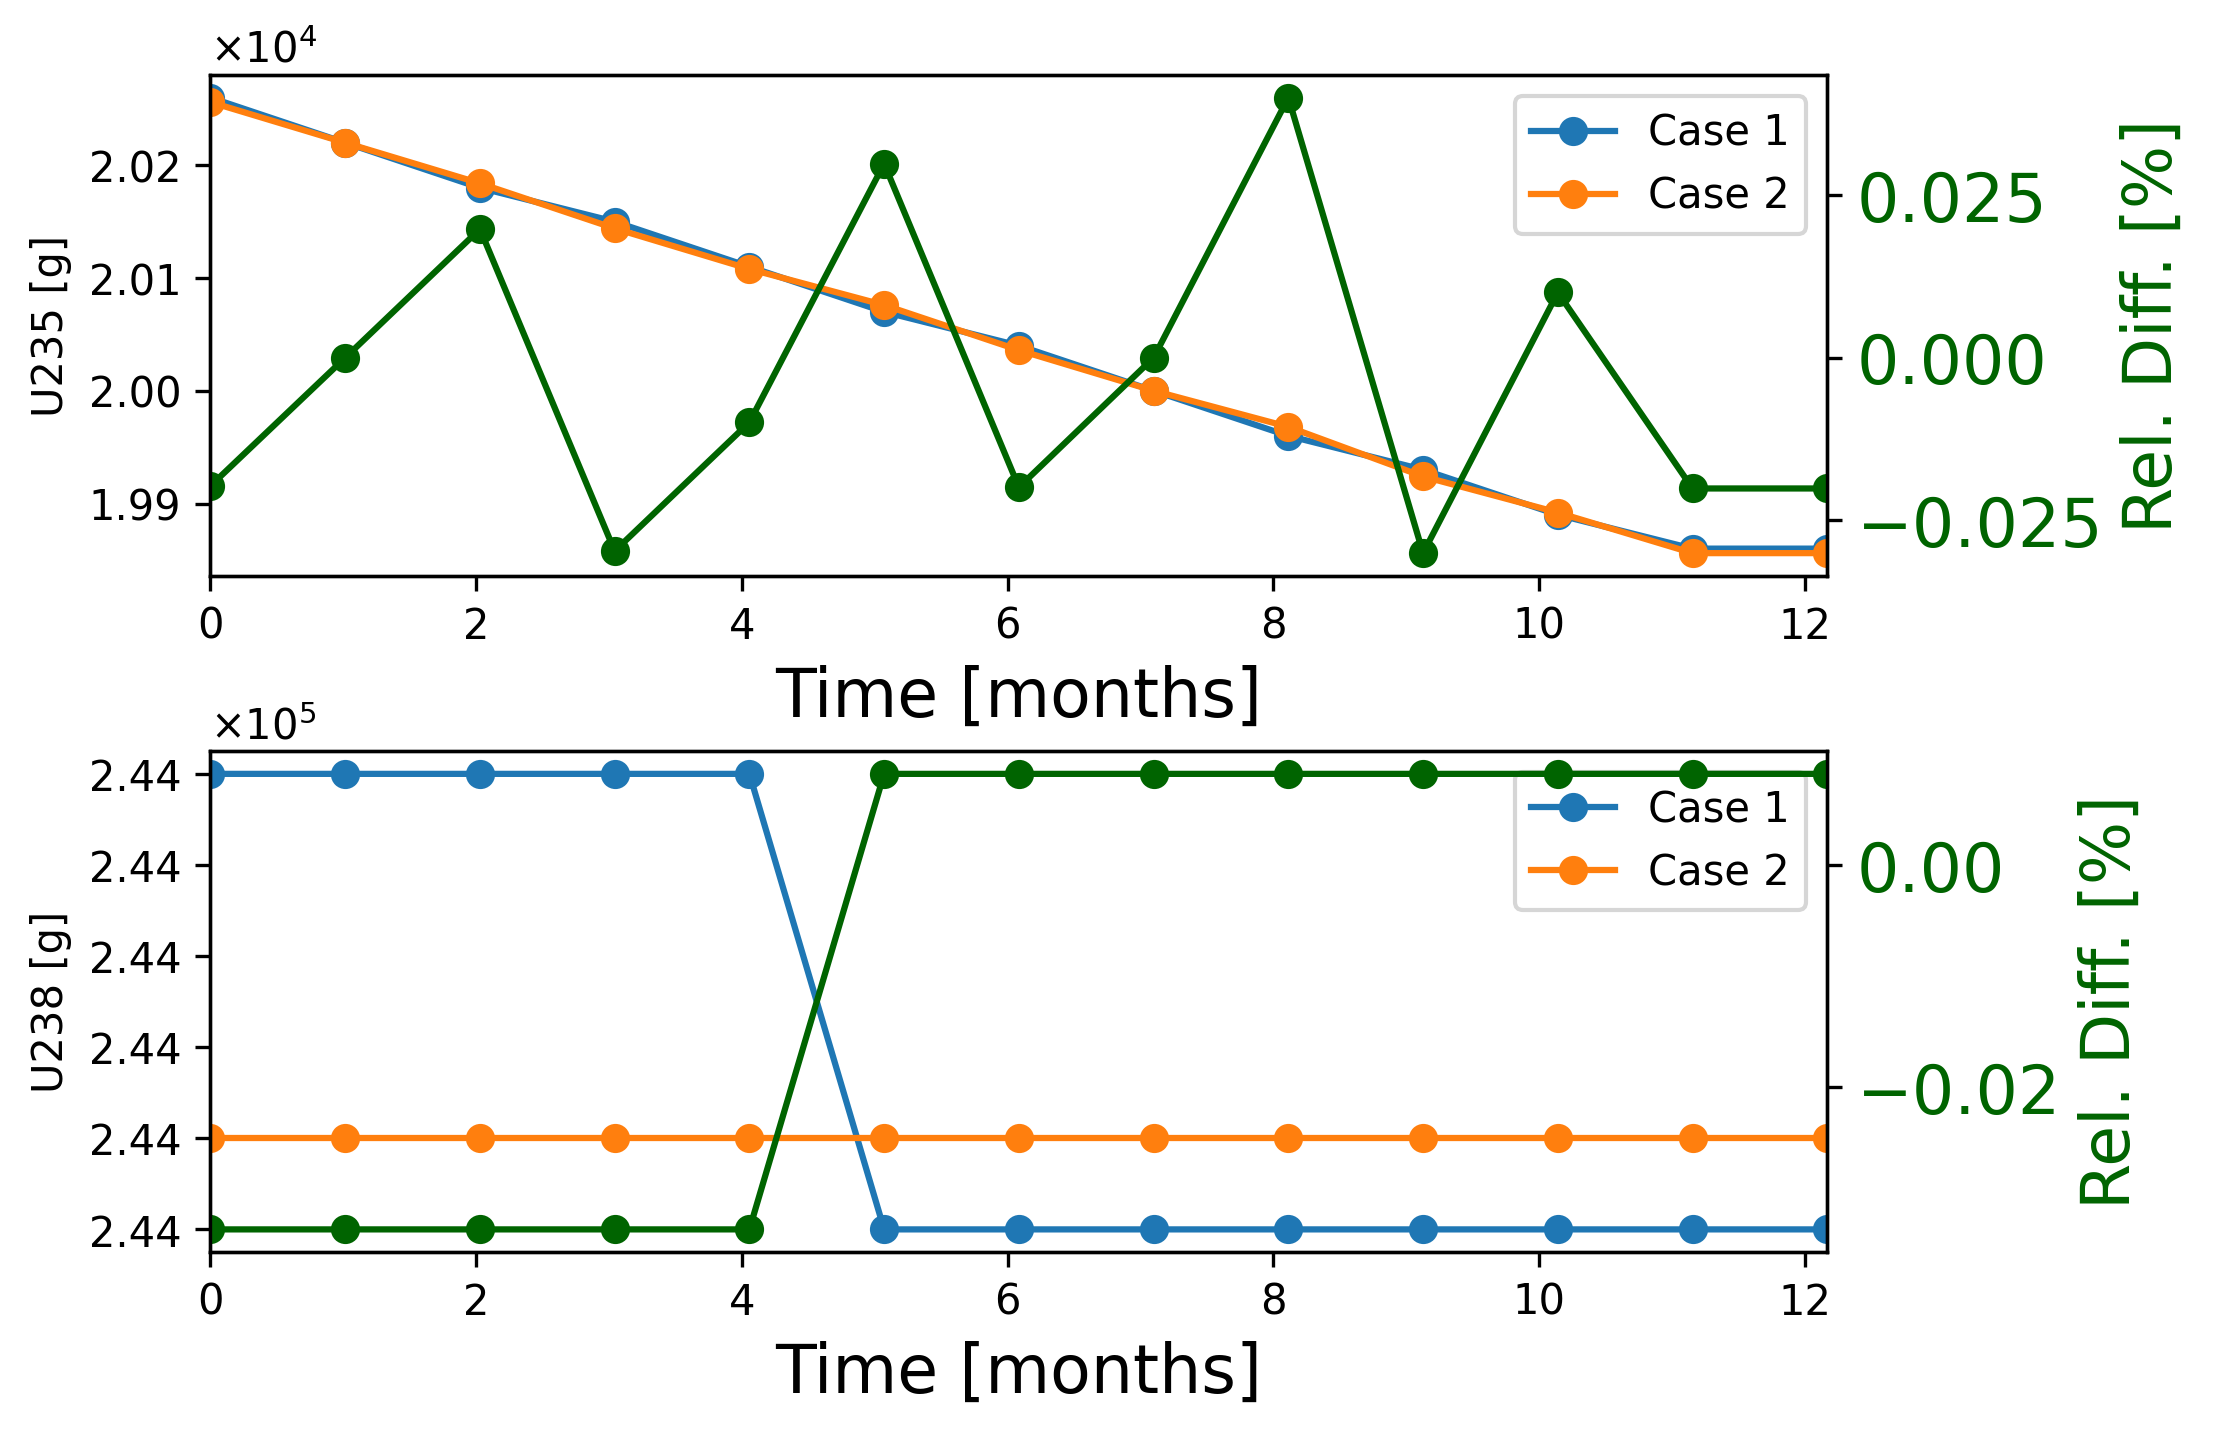
\includegraphics[width=0.98\linewidth]{figures/composition-time}
%     \hfill
%     \caption{Comparison of the uranium mass during reactor operation.}
%     \label{fig:ver-comp}
% \end{figure}

% % gamma intensity
% Figure \ref{fig:gamma-sources} displays a comparison between the repeated structures and the reference cases of the gamma source intensities in the fuel pins.
% The sources in the repeated structures' case have a uniform value across the geometry.
% The definition of the repeated structures requires the utilization of universes, and all the cells defined by the same universe are subject to the same flux level, an average value, and hence their depletion is uniform.
% The sources in the reference case are strongest in the center of the core and decrease towards the periphery, due to the flux shape, which is strongest in the center.
% Finally, given that in the repeated structures' case, the gamma source intensities are stronger in the periphery than in the reference case, and these pins contribute the most to the heating due to their proximity, the delayed heating in the core inner shell is higher.

% \begin{figure}[htbp!] %or H 
%     \centering
%     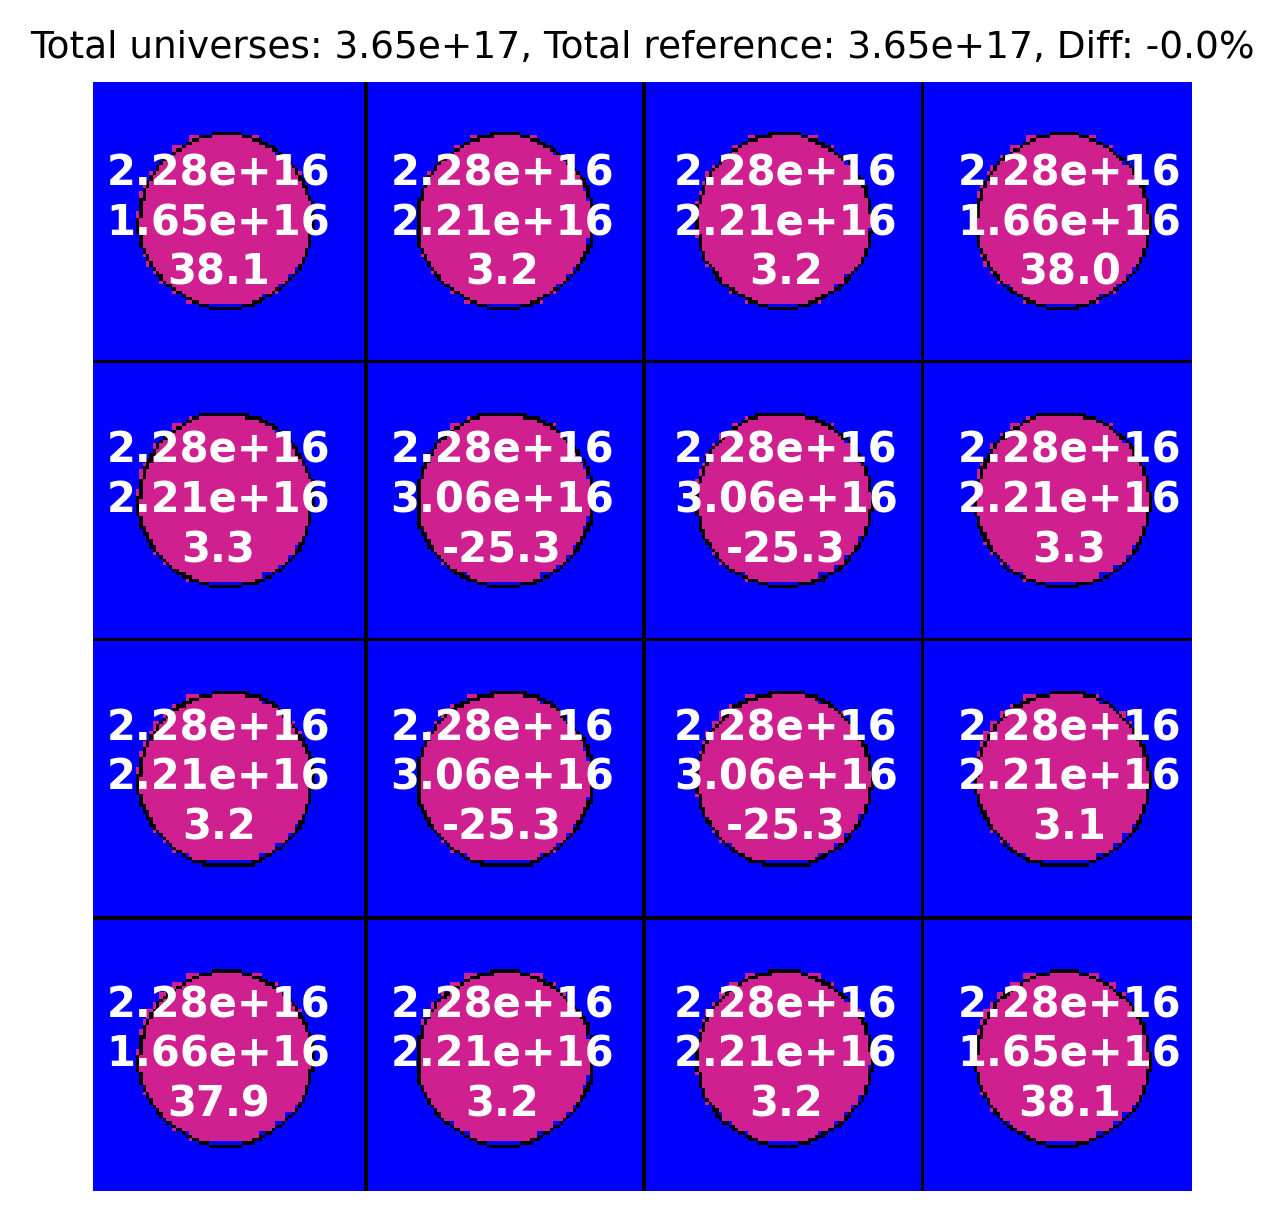
\includegraphics[width=0.80\linewidth]{figures/moaa-ref-uni-gamma-intens}
%     \hfill
%     \caption{Comparison of the intensity of the gamma sources in the fuel pins. Top value corresponds to the input file defined with repeated structures. Intermediate value corresponds to the reference intensities. Intensities expressed in decays per second. Lower value corresponds to the relative difference in \%.}
%     \label{fig:gamma-sources}
% \end{figure}

% % Conclusions from 13-
% This exercise studied the delayed heating calculation in repeated structures, such as the ones that are necessary to define HTGR models.
% Taking advantage of the MCNP input definition using repeated structures allows for simplifying the definition of cells contributing to the delayed heating/shutdown dose rates.
% Even though the results for the repeated structures' case show an overestimation of the delayed heating, the approach seems to yield a reasonable approximation.
% The results and conclusions drawn from this exercise set the path forward for the next exercises, which use the same approach for calculating the shutdown dose rate in HTGRs.

% Problem definition
% Geometry
The problem geometry is displayed in Figure \ref{fig:toy-geo2}.
The core consists of an 8x8 array of fuel pins of 1.25 cm radius with a 4 cm pitch, and it is separated from the reflector tank by an inner shell of aluminum.
The shell dimensions are an inner side length of 32 cm and 2 cm thickness.
The reflector tank is filled with light water, and its radius is 40 cm.
The whole geometry is 80 cm high.
The fuel is 7.8\%-enriched uranium with a density of 10.5 g/cm$^3$, the inner shell is made of pure aluminum with a density of 2.7 g/cm$^3$, and the water has a density of 1.0 g/cm$^3$.

\begin{figure}[htbp!] %or H 
    \centering
    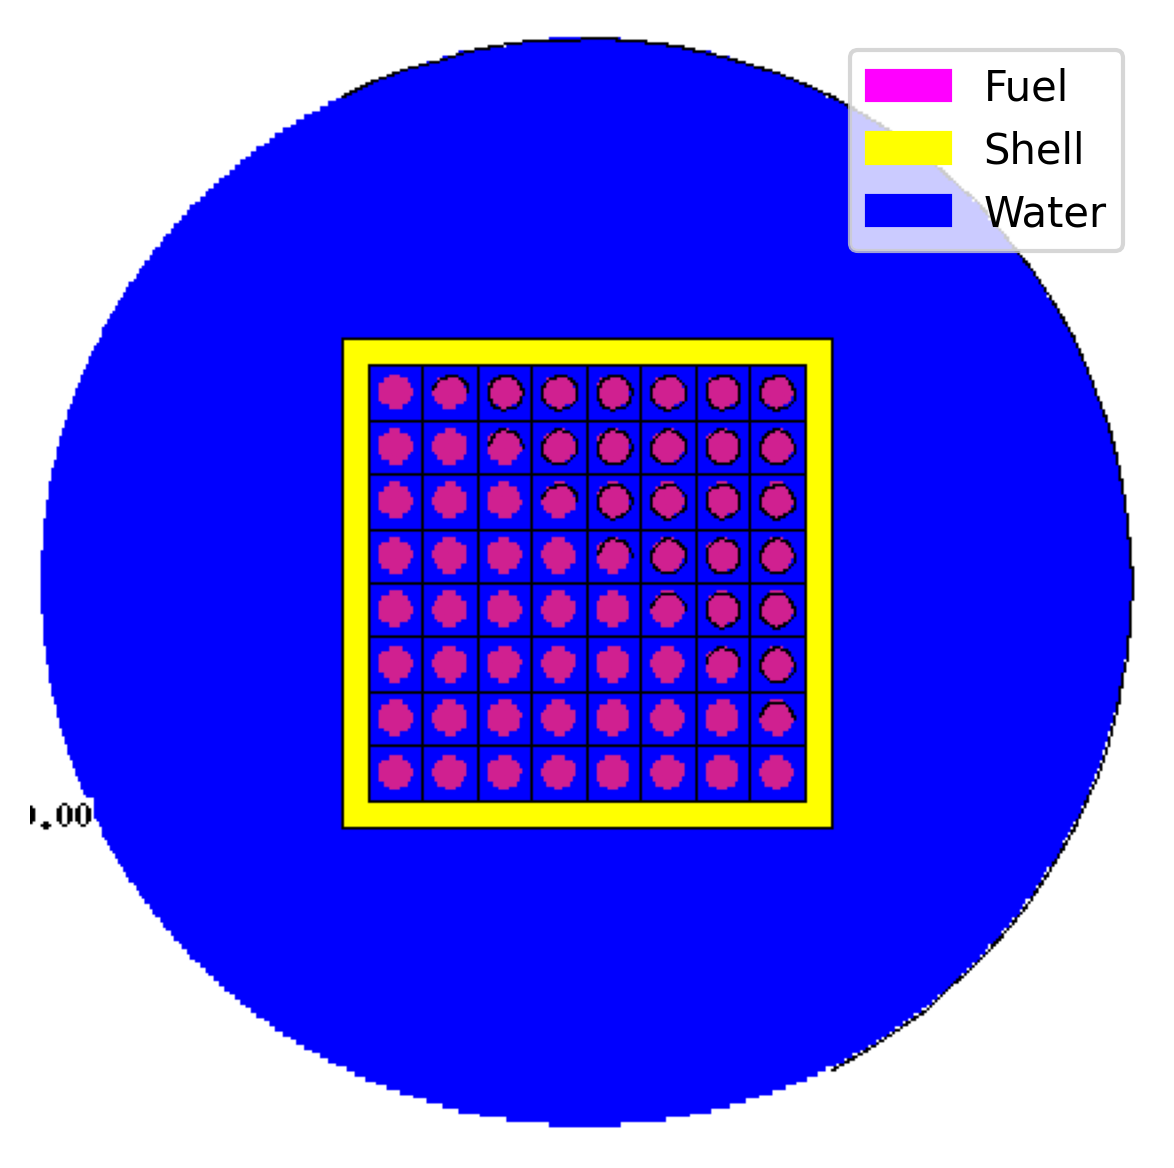
\includegraphics[width=0.6\linewidth]{figures/toy-problem-b.png}
    \hfill
    \caption{Verification problem geometry. The delayed gamma heating is calculated in the core inner shell.}
    \label{fig:toy-geo2}
\end{figure}

% The Problem
The main objective of the calculation is the estimation of the delayed gamma heating in the core inner shell, considering all the fuel pins as the radiation source.
The delayed heating is calculated after a reactor operation at a 1 MW constant power for a 12-month cycle.

% Results
Table \ref{table:verif} summarizes the main results at the end of irradiation.
While the heating equals 675.0 W in the reference case, the repeated structures' case predicts a heating of 780.4 W, which is 15.6\% larger than the reference value.
To understand this result, we need to investigate other quantities.
The average neutron flux and total photon intensity show a relative difference smaller than 0.1\%.
Figure \ref{fig:ver-comp} displays the uranium composition evolution during irradiation.
The uranium evolution displays a relative difference smaller than 0.1\%.

\begin{table}[!htb]
  \centering
  \caption{Comparison of end of irradiation integral results for the reference and repeated structure approaches.}
  \label{table:verif}
  \begin{tabular}{l|cc|c}
  \toprule
                                           & Reference  & Rep. Struct. & Rel. Diff. [\%] \\ % (RS/REF - 1)*100
  \midrule
   Delayed gamma heating [W]               & 675.0      & 780.4        & 15.6 \\
   Ave. neutron flux [10$^{13}$ n/cm2/s]   & 1.868      & 1.867        & 0.07 \\
   Tot. photon intensity [10$^{17}$ $\gamma$/s] &  3.666  &  3.668     & 0.04 \\
  \bottomrule
  \end{tabular}
\end{table}

\begin{figure}[htbp!] %or H 
    \centering
    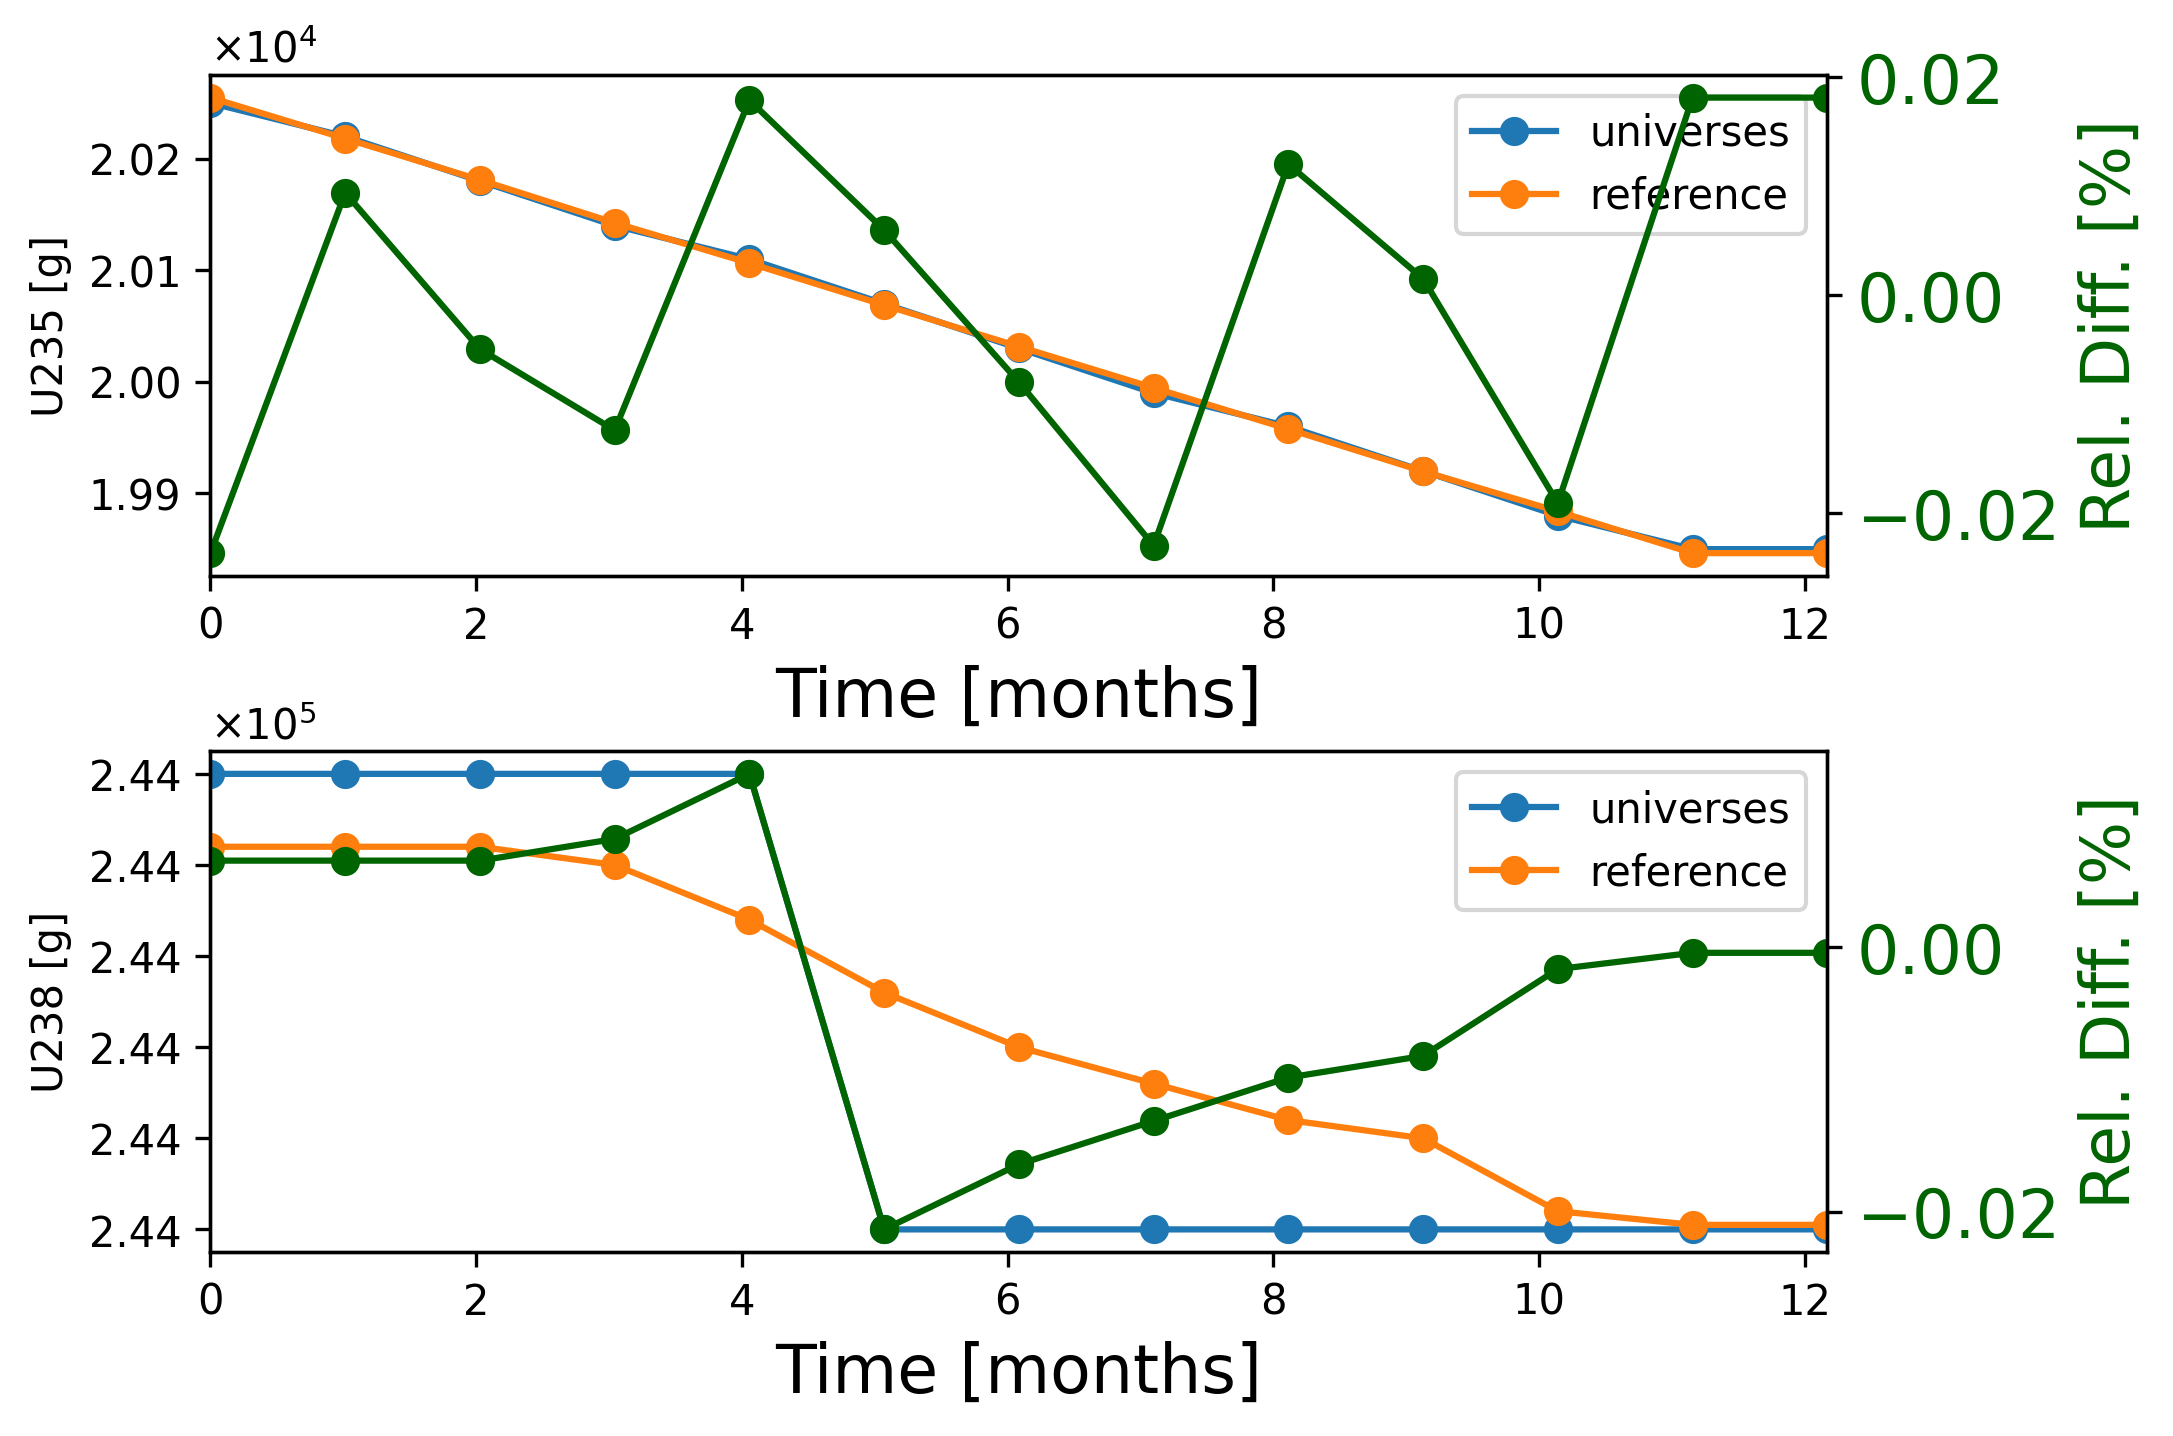
\includegraphics[width=0.65\linewidth]{figures/moaa-ref-uni-composition-time-b}
    \hfill
    \caption{Comparison of the uranium mass during reactor operation.}
    \label{fig:ver-comp}
\end{figure}

% gamma intensity
Figure \ref{fig:gamma-sources} displays a comparison between the repeated structures and the reference cases of the gamma source intensities in the fuel pins.
The sources in the repeated structures' case have a uniform value across the geometry.
The definition of the repeated structures requires the utilization of universes, and all the cells defined by the same universe are subject to the same flux level, an average value, and hence their depletion is uniform.
The sources in the reference case are strongest in the center of the core and decrease towards the periphery, due to the flux shape, which is strongest in the center.
Finally, the gamma source intensities in the repeated structures' case are stronger in the periphery than in the reference case.
As these pins contribute the most to the heating of the shell due to their proximity, the delayed heating in the core inner shell is higher.

\begin{figure}[htbp!] %or H 
    \centering
    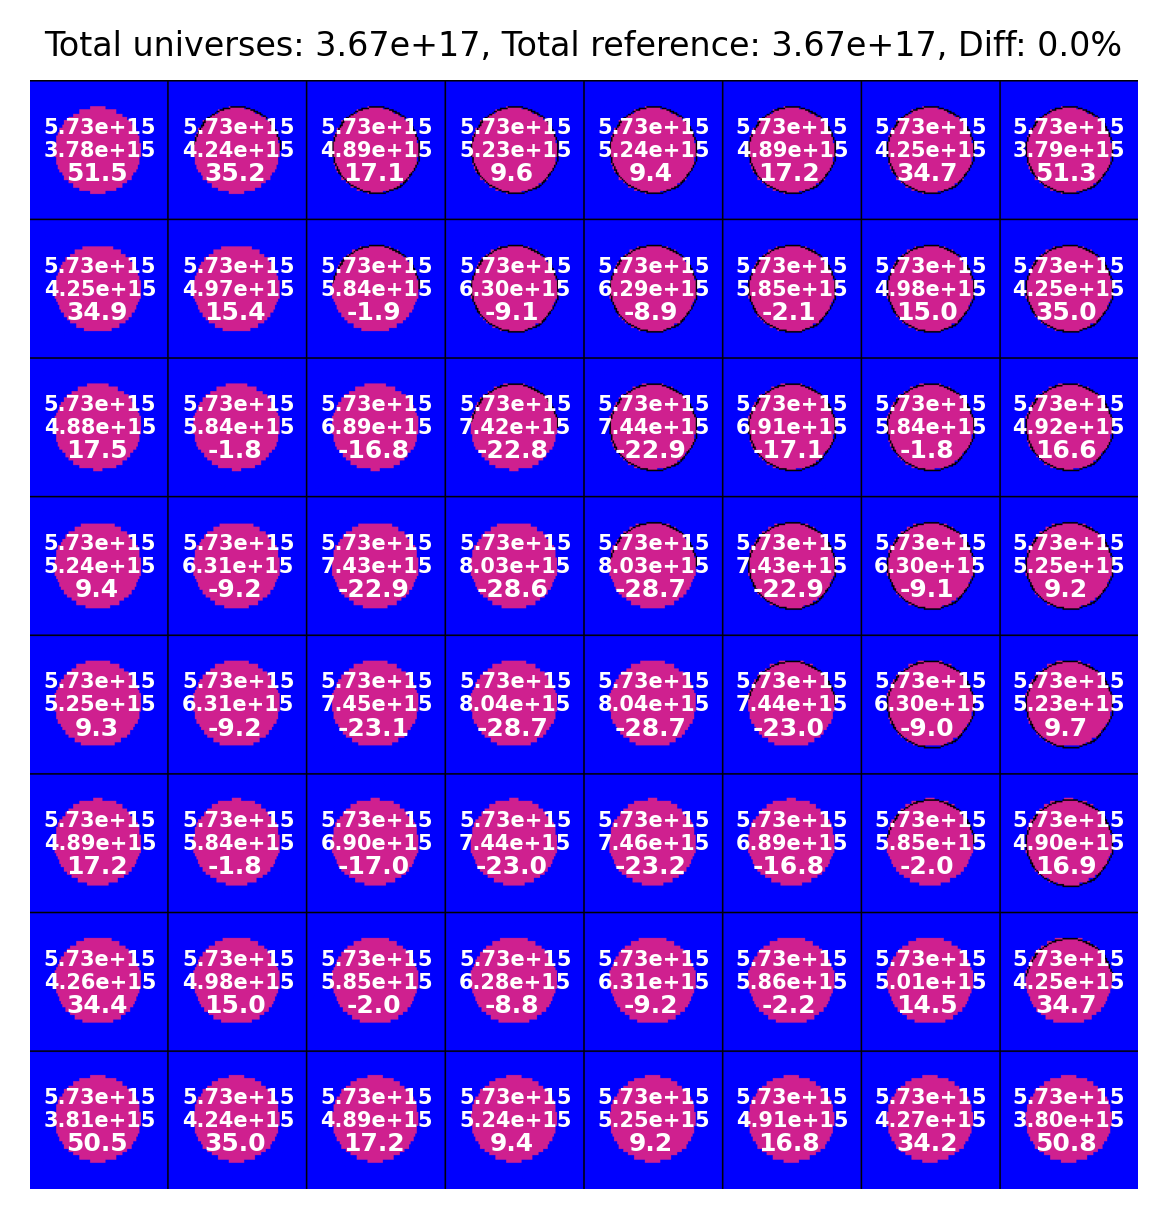
\includegraphics[width=0.65\linewidth]{figures/moaa-ref-uni-gamma-intens-b}
    \hfill
    \caption{Comparison of the intensity of the gamma sources in the fuel pins. The top value corresponds to the repeated structure approach. The intermediate value corresponds to the reference values. Intensities expressed in decays per second. The lower value corresponds to the relative difference in \%.}
    \label{fig:gamma-sources}
\end{figure}

As shown in Figure \ref{fig:gamma-sources}, the accuracy of the repeated structure approach is affected when the problem shows a strong spatial effect.
This suggests that using a repeated structure that comprehends the whole core is not the right approach.
Instead, a better approach would consider the flux shape variation to choose the repeated structures.
This exercise was also conducted using repeated structures but arranging the fuel pins in groups of 4.
Table \ref{table:verif2} displays the results for that case.
The relative difference for the delayed gamma heating is 4.3\%, while the rest of the results do not change considerably.
The results show that grouping the structures based on the location, and hence similar flux levels, yields better results.

\begin{table}[!htb]
  \centering
  \caption{Comparison of end of irradiation integral results for the reference and repeated structure approaches.}
  \label{table:verif2}
  \begin{tabular}{l|cc|c}
  \toprule
                                           & Reference  & Rep. Struct. & Rel. Diff. [\%] \\ % (RS/REF - 1)*100
  \midrule
   Delayed gamma heating [W]               & 675.0       & 704.3       &  4.3  \\
   Ave. neutron flux [10$^{13}$ n/cm2/s]   & 1.868       & 1.867       & -0.03 \\
   Tot. photon intensity [10$^{17}$ $\gamma$/s] &  3.666 & 3.667       &  0.03 \\
  \bottomrule
  \end{tabular}
\end{table}

% Conclusions from 13-
This exercise studied the delayed heating calculation in repeated structures, such as the ones that are necessary to define HTGR models.
Taking advantage of the MCNP input definition using repeated structures allows for simplifying the definition of cells contributing to the delayed heating/shutdown dose rates.
Even though the results for the repeated structures' case show an overestimation of the delayed heating, the approach yields a reasonable approximation when considering the flux spatial variation.
The results and conclusions drawn from this exercise set the path forward for the next exercises, which use the same approach for calculating the shutdown dose rate in HTGRs.


\section{AGR-1}
\label{sec:agr}

% Depletion results: AGR1 benchmark

% AGR-1
The \gls*{AGR1} \cite{sterbentz_agr1_2018} was a TRISO-particle irradiation test in the \gls*{ATR}, a 250-MWth high flux test reactor located at the Reactor Technology Complex of the \gls*{INL}.
This experiment was part of the \gls*{DOE} Advanced Gas Reactor Fuel Development and Qualification Program to support the \gls*{NGNP} program.

% ATR: reactor description
Figure \ref{fig:atrq} shows the MCNP quarter model of ATR, which represents the core east quadrant, which is used for the simulations.
This model simplifies the reactor geometry by grouping the fuel plates into three radial zones.
% AGR-1 in ATR
The AGR-1 experiment was placed in the B-10 position and irradiated over 13 power cycles for a period corresponding to three years.

% ATR figure of the model
\begin{figure}[htbp!] %or H 
    \centering
    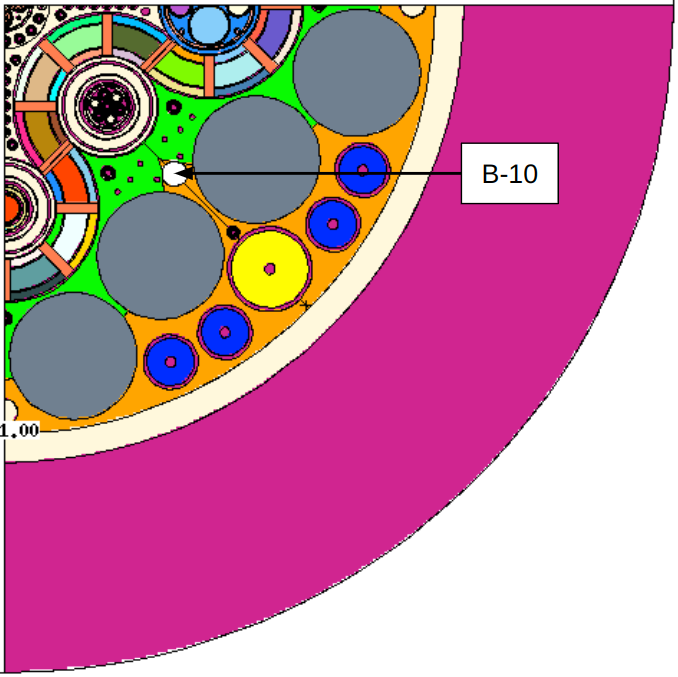
\includegraphics[width=0.70\linewidth]{figures/atr-quarter2}
    \hfill
    \caption{MCNP quarter model of ATR.}
    \label{fig:atrq}
\end{figure}

% Benchmark
The AGR-1 Depletion Benchmark \cite{sterbentz_agr1_2018} describes the experiment test train, shown in Figure \ref{fig:agr-geo}.
The test train consists of six cylindrical capsules vertically stacked, wherein the compacts are separated into three columns, with each column containing four compacts, adding up to a total of 72 compacts.
The experiment includes four different types of compact.
Capsules 3 and 6 contain the baseline compact, capsule 5 contains variant 1, capsule 2 contains variant 2, and capsules 1 and 4 contain variant 3.
The difference between compact types is that the particle layers change slightly in thickness and density, while the fuel kernel remains the same.
Additionally, each type of compact has a different number of embedded particles.
The main model simplifications are that the hafnium (Hf) shroud surrounds the whole circumference of the capsule, the gas lines, thermocouples, and thru-tubes are neglected, and the TRISO particles are arranged in a regular lattice.

\begin{figure}[htbp!] %or H
  \centering
  \begin{subfigure}{0.49\textwidth}
    \centering
    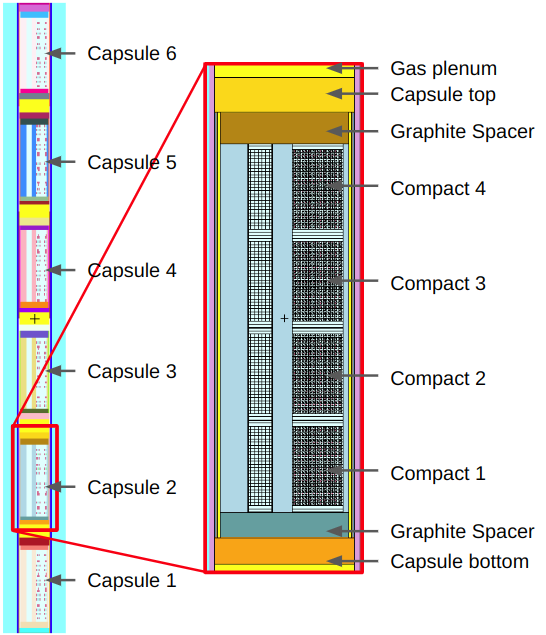
\includegraphics[width=0.9\linewidth]{figures/agr-paper-1}
    \caption{Axial view.}
    \label{fig:agr-a}
  \end{subfigure}
  \begin{subfigure}{0.49\textwidth}
    \centering
    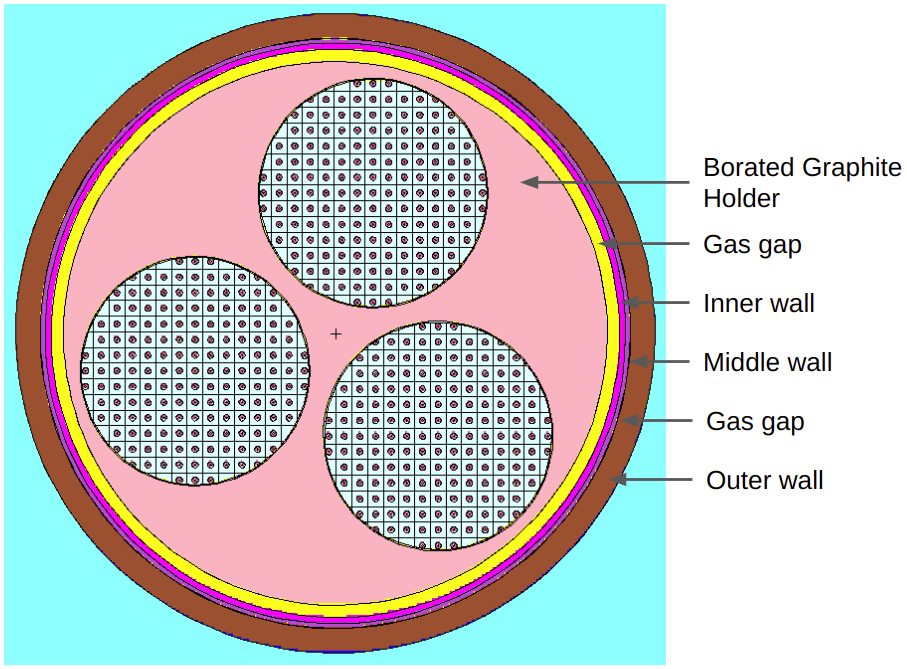
\includegraphics[width=0.9\linewidth]{figures/agr-paper-2}
    \caption{Top view.}
    \label{fig:agr-b}
  \end{subfigure}
  \caption[benchmark]{AGR-1 experiment geometry.}
  \label{fig:agr-geo}
\end{figure}

% \begin{figure}[htbp!] %or H 
%     \centering
%     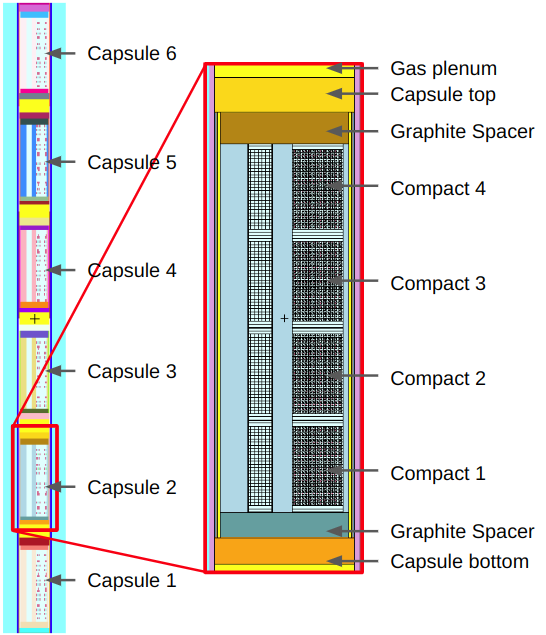
\includegraphics[width=0.90\linewidth]{figures/agr-paper-1}
%     \hfill
%     \caption{Axial view of the AGR-1 experiment.}
%     \label{fig:agr-1}
% \end{figure}

% \begin{figure}[htbp!] %or H 
%     \centering
%     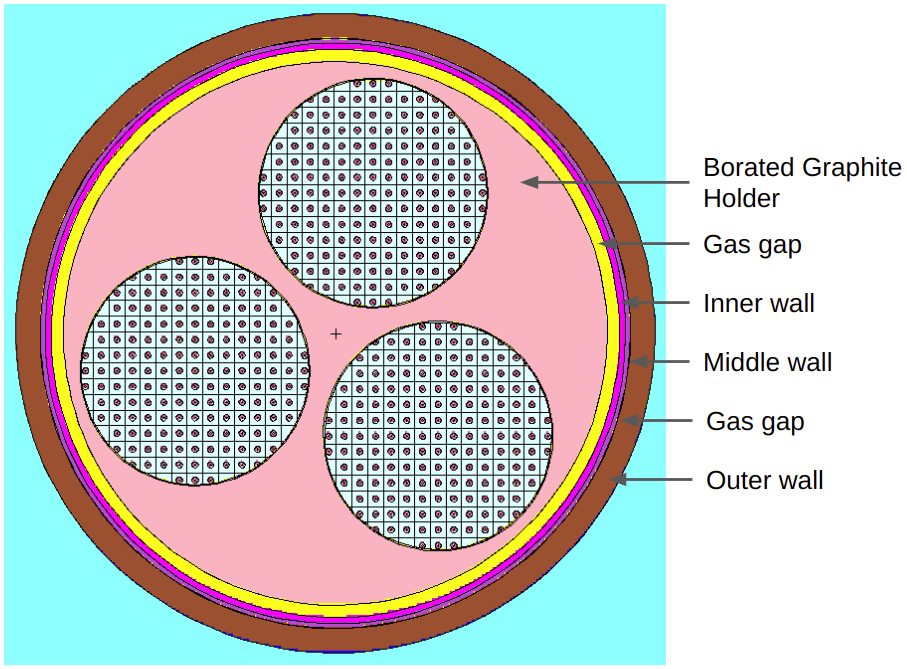
\includegraphics[width=0.90\linewidth]{figures/agr-paper-2}
%     \hfill
%     \caption{Top view of the AGR-1 experiment.}
%     \label{fig:agr-2}
% \end{figure}

The benchmark data includes for each time step: the lobe power, the OSCC positions, and the neck shim insertion condition.
Figure \ref{fig:agr-data} shows the benchmark data for the first irradiation cycle or cycle 138B.
Because the data includes 662 time steps, and to reduce the complexity of the model, this work considers the power, OSCC position, and neck shim insertion condition to take the cycle average value.
For the neck shim insertion, the average value is considered the cycle predominant insertion condition.
For example, if the NE 1 rod is inserted through most of the cycle, this work assumes that it is inserted throughout the whole cycle length.
For tally normalization, the B-10 position tally data is typically normalized to an east lobe power defined as the average of the northeast, center, and southeast lobe powers.
For the fuel composition, the MCNP model defines the driver fuel for the \gls*{BOC} 145A and assumes it to be appropriate for the \gls*{BOC} of all the cycles.
This work takes that assumption one step further and considers the driver fuel composition to remain constant during all the simulations.

\begin{figure}[htbp!] %or H
  \centering
  \begin{subfigure}{1\textwidth}
    \centering
    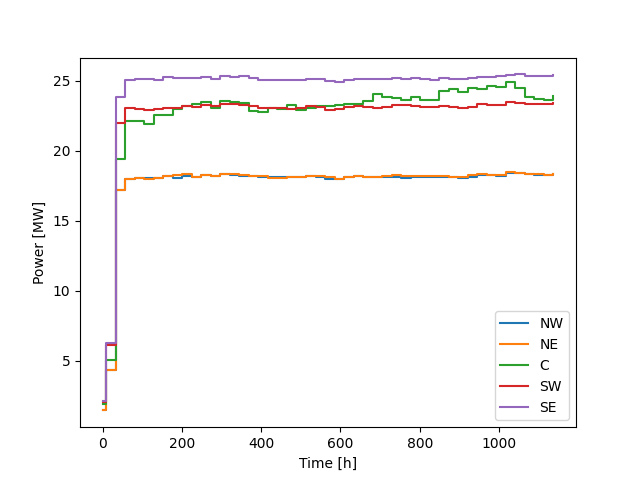
\includegraphics[width=0.55\linewidth]{figures/power_cycle_138B}
    \caption{Lobe power.}
    \label{fig:agrd-a}
  \end{subfigure}
  \begin{subfigure}{1\textwidth}
    \centering
    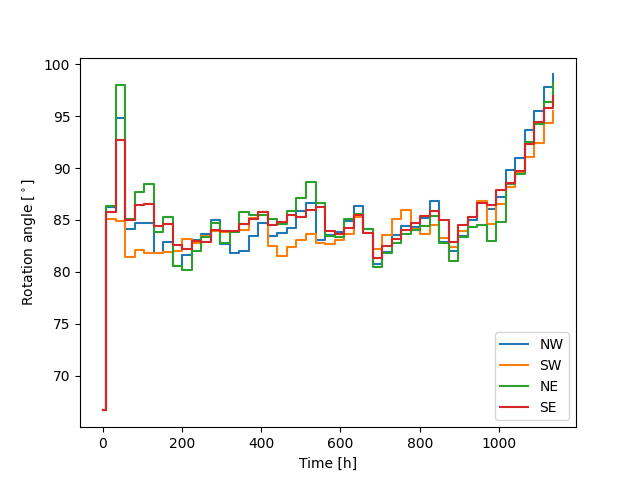
\includegraphics[width=0.55\linewidth]{figures/oscc_cycle_138B}
    \caption{OSCC rotation angle.}
    \label{fig:agrd-b}
  \end{subfigure}
  \begin{subfigure}{1\textwidth}
    \centering
    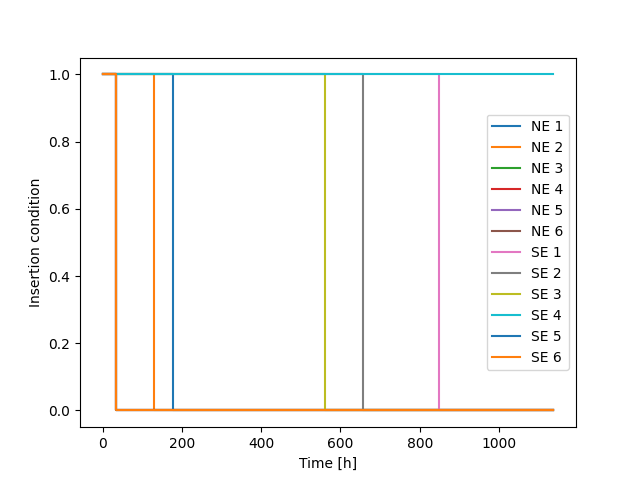
\includegraphics[width=0.55\linewidth]{figures/neck_cycle_138B}
    \caption{Neck shim insertion condition, where $0/1$ means withdrawn/inserted.}
    \label{fig:agrd-c}
  \end{subfigure}
  \caption[benchmark]{AGR-1 benchmark data for first irradiation cycle (cycle 138B).}
  \label{fig:agr-data}
\end{figure}


% Results
Figure \ref{fig:agr-deplet} displays the experiment burnup as a function of the axial position.
This figure compares this work's results versus the benchmark results.
As the raw data from benchmark results are not available, this figure shows both results overlapped, allowing for the visualization of the following phenomena.
The benchmark results include more data points than this work.
While the benchmark subdivides each capsule into eight pieces, this work considers only one average value.
Stacks 1 and 2 show the largest burnup values, as they are the closest to the reactor center.
This work results agree on this aspect with the benchmark results.
The burnup shape for each capsule displays higher values in the bottom and top ends.
The reason for this is the presence of the graphite spacers in the bottom and top regions of each capsule.
This result is also consistent with the benchmark results.
Finally, this work predicts a lower burnup than the benchmark results.
The reason for this is the modeling simplification of considering the average values for each cycle, and most importantly, utilizing the cycle average power.
Although not shown here, some cycles include a reactor shutdown, in which the reactor total power becomes zero (even for 40 days).
For these cycles, the average cycle values simplification is expected to underpredict the cycle burnup.
For future reference, this simplification should not be used when trying to follow the benchmark formally.
However, for the purpose of this work focusing on shutdown dose rates, this simplification and consistent results are deemed valid. 

\begin{figure}[htbp!] %or H 
    \centering
    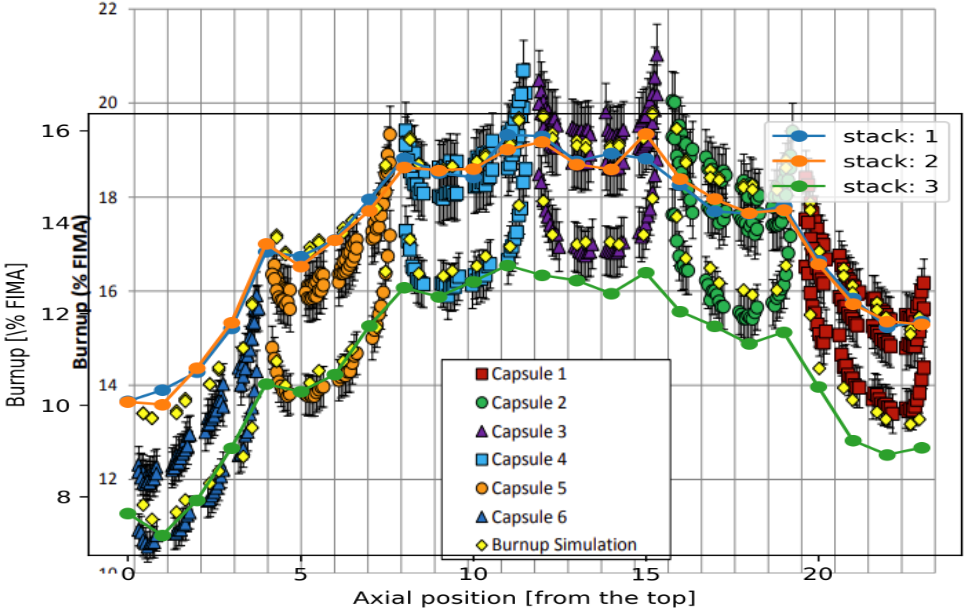
\includegraphics[width=0.9\linewidth]{figures/agr-depletion}
    \hfill
    \caption{AGR-1 experiment burnup as a function of the axial position.}
    \label{fig:agr-deplet}
\end{figure}

Table \ref{table:agr-contr} shows the contribution from all the photon sources at different decay times.
The graphite spacers and holders have the smallest contribution.
The holders contain boron and hence have a higher contribution than the spacers.
After one day, the largest contribution comes from fuel at 53.19\% followed by the Hf shroud with a contribution of 41.64\%.
After 30 days, the contribution from the fuel decreases to 30.03\% while the Hf shroud contribution of 62.11\% becomes predominant.
After 365 days, the Hf shroud contribution drops, and the largest contributor becomes the fuel at 56.95\%, followed by the structures of stainless steel which add up to 42.54\%. 
The total source intensities decrease two orders of magnitude after a 365-day decay.

\begin{table}[!htb]
  \centering
  \caption{Photon source contribution by decay time.}
  \label{table:agr-contr} 
  \begin{tabular}{lcccc}
  \toprule
  Contribution                 & Units  & 1 day        & 30 days        & 365 days      \\
  \midrule
  Fuel                         & \%     & 53.19         & 30.03          & 56.95         \\
  Bottom support SS316L        & \%     & 0.76          & 1.17           & 6.47          \\
  Inner wall SS316L            & \%     & 0.43          & 0.63           & 3.07          \\
  Top support SS316L           & \%     & 0.85          & 1.3            & 7.10          \\
  Outer wall SS316L            & \%     & 3.13          & 4.77           & 25.9          \\
  Low graphite spacer          & \%     & 6.93$\times$10$^{-10}$  & 2.56$\times$10$^{-9}$  & 6.37$\times$10$^{-8}$  \\
  Upper graphite spacer        & \%     & 8.04$\times$10$^{-10}$  & 2.96$\times$10$^{-9}$  & 7.38$\times$10$^{-8}$  \\
  Borated graphite holder      & \%     & 7.59$\times$10$^{-7}$   & 2.77$\times$10$^{-6}$  & 6.14$\times$10$^{-5}$  \\
  Hf shroud                    & \%     & 41.64         & 62.11          & 0.50          \\ \hline
  Total                        & $\gamma$/s  & 1.199$\times$10$^{15}$  & 3.2529$\times$10$^{14}$  & 1.305$\times$10$^{13}$  \\
  \bottomrule
\end{tabular}
\end{table}

% Figure \ref{fig:agr-dose} displays the dose rate surrounding the AGR test train during the \gls*{PIE}.
% The dose rate is calculated for the experiment located in a 1x1 m box at different decay times.
% % shape:
% The dose rate is plotted over the red line shown in the 2D plot, and as expected it has a $1/r^2$ shape.
% The highest value is in the proximity of the experiment for all the decay times.
% % max values over time
% After one day, the highest value is greater than 600 Sv/h, and it decreases to 30 Sv/h at 1 m from the experiment.
% After 30 days, the values are reduced about four times, and the highest value is slightly greater than 175 Sv/h, and it decreases to 5 Sv/h at 1 m from the experiment.
% After 365 days, the values are reduced about 200 times, and the highest value is slightly greater than 3.5 Sv/h, and it decreases to 0.2 Sv/h at 1 m from the experiment.

% \begin{figure}[htbp!] %or H
%   \centering
%   \begin{subfigure}{.9\textwidth}
%     \centering
%     \includegraphics[width=1\linewidth]{dose_1}
%     \caption{}
%   \end{subfigure}
%   \begin{subfigure}{.9\textwidth}
%     \centering
%     \includegraphics[width=1\linewidth]{dose_30}
%     \caption{}
%   \end{subfigure}
%   \begin{subfigure}{.9\textwidth}
%     \centering
%     \includegraphics[width=1\linewidth]{dose_365}
%     \caption{}
%   \end{subfigure}
%   \caption[Three solutions]{Dose rate for the PIE of AGR in a 1x1 m room and the values over the line denoted in red. Dose rates for different decay times: (a) 1 day, (b) 30 days, (c) 365 days.}
%   \label{fig:agr-dose}
% \end{figure}

Table \ref{table:agr-dose} shows the dose rate at different distances from the center of the AGR test train by decay time.
% Discussion
The results show that even after one year decay, and at 98 cm distance from the experiment, the exposure from the experiment decay is high.
For that reason, the experiment \gls*{PIE} would need to await more than 1 year to be conducted or utilize a hot cell with the appropriate shielding to prevent any unnecessary exposure of the personnel.

\begin{table}[!htb]
  \centering
  \caption{Dose rate at different distances from the center of the experiment by decay time. Values expressed in Sv/h.}
  \label{table:agr-dose} 
  \begin{tabular}{lcccc}
  \toprule
  Distance   & 1 day        & 30 days        & 365 days      \\
  \midrule
  6 cm       & 666.2         & 190.3          & 3.7           \\
  46 cm      & 72.7          & 20.4           & 0.4           \\
  98 cm      & 25.4          & 7.3            & 0.1           \\
  \bottomrule
\end{tabular}
\end{table}


\section{The $\mu$HTGR}
\label{sec:micro}


% Intro to HTGRs
% Motivation - from 12-
\Glspl*{HTGR} have gained a lot of attention in the past few decades.
% VHTR 
In 2002, the \gls*{VHTR} was proposed as one of the Generation-IV nuclear energy systems for the co-generation of electricity and hydrogen \cite{doe_vhtr_2002}.
% NGNP
In 2006, the \gls*{DOE} and the \gls*{INL} established the \gls*{NGNP} project to develop, license, build, and operate a prototype modular \gls*{HTGR} to produce hydrogen while generating electric power \cite{ngnp}.
% Add more examples of HTGRs built/developed in the past couple of decades, maybe another micro-reactor ?
More recent examples of HTGRs are new microreactor designs.
% StarCore
StarCore Nuclear has partnered with the local government of Pinawa, Canada to demonstrate the powering of off-grid communities and mining companies with an HTGR \cite{starcore}.
% BWXT
The \gls*{DOD} has recently awarded a contract to BWXT to deliver a transportable 1-5 MWe HTGR to be completed and delivered by 2024 \cite{bwxt}.
% USNC
The \gls*{UIUC} has partnered with the \gls*{USNC} to build a microreactor on its campus, a 10 MWth \gls*{HTGR} \cite{uiuc-mmr2}.
The new reactor facility will offer UIUC a diverse set of opportunities for research, including instrumentation and control, multi-physics validation, reactor prototype testing, and micro-grid operations.

HTGR technology presents many distinct features from the current \gls*{LWR} fleet, and potential decommissioning strategies should take them into consideration.
After reactor shutdown, the ongoing decay may inflict dose on workers and equipment in the reactor surroundings.
In \glspl*{LWR}, the common strategy entails flooding the entire reactor cavity to remove the spent fuel, as the water column between the assemblies and the operators provides enough shielding.
% High-temperature graphite oxidation
HTGRs cannot, however, implement such a strategy because of the presence of large volumes of high-temperature graphite in the core, and this could lead to graphite oxidation \cite{oxidation}, degrading its structural and functional properties.
Nevertheless, the proper characterization of the shutdown dose rates can guide establishing a suitable decommissioning strategy.

% % More motivation
% Furthermore, some of the microreactor designs envision core lifetimes of more than 10 years, which will allow their continuous operation without refueling outages \cite{usnc_mmr}.
% On the other hand, a long reactor lifetime is a feature that may require additional planning.
% A long reactor lifetime may bring along a high activation of the core components, requiring modeling capabilities to determine suitable decommissioning strategies.

% % Even more motivation, is similar to what I described above
% % ho_calculation_2022
% Decay gamma and its equivalent dose rate are also one of the important factors for safely conducting various works after reactor shutdown such as periodic maintenance, fuel shuffling, removing spent fuel at the end of cycle, etc.
% Therefore, the information of decay gamma distribution in the entire core would also be beneficial to optimize the shielding design of the HTGR.



% Intro
This exercise uses the shutdown dose rate calculation workflow described above to study a decommissioning strategy for a model based on an early version of the \gls*{USNC} \gls*{MMR} design \cite{uiuc-mmr2}, hereby referred to as $\mu$HTGR \cite{fairhurst_sdr_2023}.
Because most of the technical details of the MMR are not public, the $\mu$HTGR model is based on the publicly available information of the reactor \cite{uiuc-mmr2, usnc_mmr, chalk_mmr, neup_mmr}.

The decommissioning strategy places the reactor in a safe shutdown state and allows it to cool down for three months \cite{usnc_mmr}.
The plan continues with the removal of the reactor lid at the citadel floor, control rod driving mechanisms, \gls*{RPV} lid, and upper core restraint structures to allow for the fuel assembly unloading before removing the vessel itself.
This exercise intends to quantify the dose rate that a worker would experience if standing at ground level on the citadel floor above the reactor top while the reactor core is exposed.

% Problem definition
Figure \ref{fig:model-1} displays the $\mu$HTGR core layout.
The core region consists of 24 fuel assemblies, 12 control assemblies, and one reserved shutdown assembly in the center.
The assembly pitch is 30 cm.
Four layers of assemblies stacked on top of each other encompass the core in the axial direction.
Additionally, the reactor has a radial, bottom, and top reflectors of graphite.
The assemblies and the bottom and top reflectors are 68 cm high and the radial reflector has a 134 cm radius.
The model considers a graphite density of 1.75 g/cm$^3$ for the assemblies and reflector regions.
% The assemblies
Within the assemblies, the fuel and coolant channels have 1.15 cm and 0.775 cm radius, respectively, with a channel pitch of 3.2 cm.
While each control assembly has a 4 cm-radius control rod hole, the reserved shutdown assembly has a 6 cm-radius control rod hole.

\begin{figure}[htbp!]
  \begin{center}
    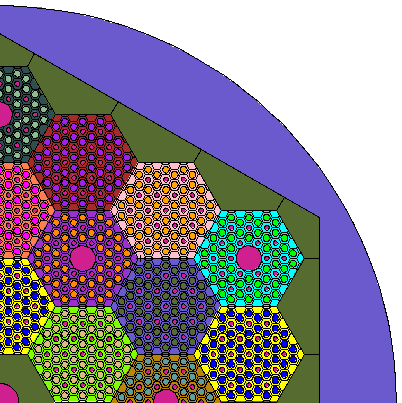
\includegraphics[width=0.60\linewidth]{figures/mcnp-diagram-1}
  \end{center}
  \caption{Quarter section of the $\mu$HTGR core.}
  \label{fig:model-1}
\end{figure}

% The compact
A column of fuel compacts fills out each fuel channel.
The compacts are made of SiC, have a density of 3.2 g/cm$^3$, and hold TRISO particles with a 40\% packing fraction.
The model considers the particles to be uniformly distributed with a particle pitch of 0.1 cm.
Table \ref{table:description} summarizes the characteristics of the TRISO particles.

\begin{table}[!htb]
  \centering
  \caption{TRISO particle definition.}
  \label{table:description} 
  \begin{tabular}{cccc}
  \toprule
   Layer  & Thickness [cm] & Material & Density [g/cm$^3$] \\
  \midrule
   Kernel & 0.0250 & UO2 ($\varepsilon$=19.75\%) & 10.8 \\
   Buffer & 0.0100 & C & 0.98 \\
   IPyC   & 0.0040 & C & 1.85 \\
   SiC    & 0.0035 & SiC & 3.20 \\
   OPyC   & 0.0040 & C & 1.86 \\
  \bottomrule
  \end{tabular}
\end{table}

% SDR calculations
Figure \ref{fig:model-2} displays the side view of the MCNP model.
In the radial direction, the model neglects the presence of the RPV side wall and considers the reactor to be in a cavity of Portland concrete (2.3 g/cm$^3$ density).
The concrete wall is located 191 cm away from the radial reflector and has a 100 cm-thickness.
In the axial direction, the cavity is limited by the citadel floor of Portland concrete with a 70 cm-thickness.
The distance from the top of the reactor to the citadel floor (ground level) is 700 cm.
The remaining volumes are filled with air (80 vol\% nitrogen, 20 vol\% oxygen).

\begin{figure}[htbp!]
  \begin{center}
    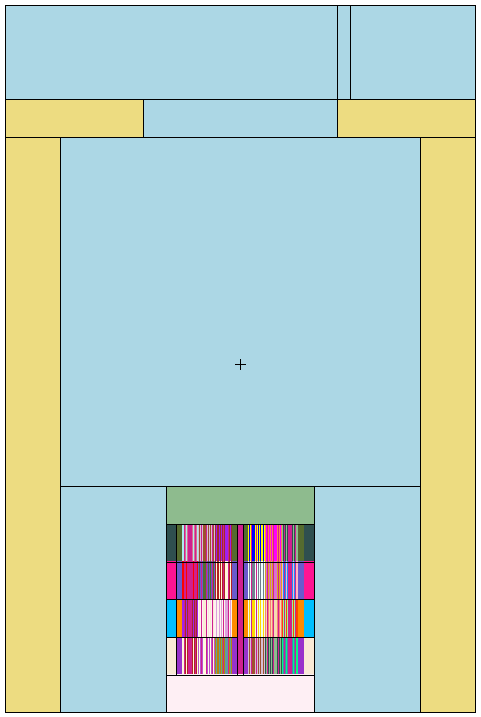
\includegraphics[width=0.40\linewidth]{figures/mcnp-diagram-2}
  \end{center}
  \caption{Side view of the MCNP model including reactor core, reactor cavity, side walls, and citadel.}
  \label{fig:model-2}
\end{figure}

The dose rate is calculated for a worker standing at ground level on the citadel floor.
The calculations use a standard person (often called ``reference man'') of 70 kg weight and 170 cm height, which is represented by an equivalent cylinder.
Considering an average human density of 0.985 g/cm$^3$ yields an equivalent cylinder of 11.53 cm radius.

The calculations consider as radiation sources the fuel in the TRISO particles in all the assemblies and the bottom, top, and radial reflectors.
A sensitivity study determined that the radiation contribution from the fuel particles is approximately 8 orders of magnitude larger than the contribution from the graphite in the assemblies.
The TRISO particle contribution is separated by assembly, for which each assembly has an independent depletion.
% CHANGES IN MCNP INPUT
% To accommodate the MOAA calculations, the MCNP input file took into account the following considerations.
% First, each assembly had an independent material definition in the MCNP input file to allow for their independent depletion.
Finally, the isotope definitions in the MCNP model used the ENDF/B-VIII.0 cross-sections at room temperature.

% Results
% Burnup results
Figure \ref{fig:res-1} displays the $K_{eff}$ time evolution.
The core has an initial $K_{eff}$ of 1.26797 and reaches the end of life at 16.07 years.
Although the original reactor is expected to run for 20 years, the $\mu$HTGR is a simplified version and several of its defining parameters are assumed, as the original parameters are not publicly available.
However, for the purposes of this discussion, the assumptions considered yield an adequate model.

\begin{figure}[htbp!]
  \begin{center}
    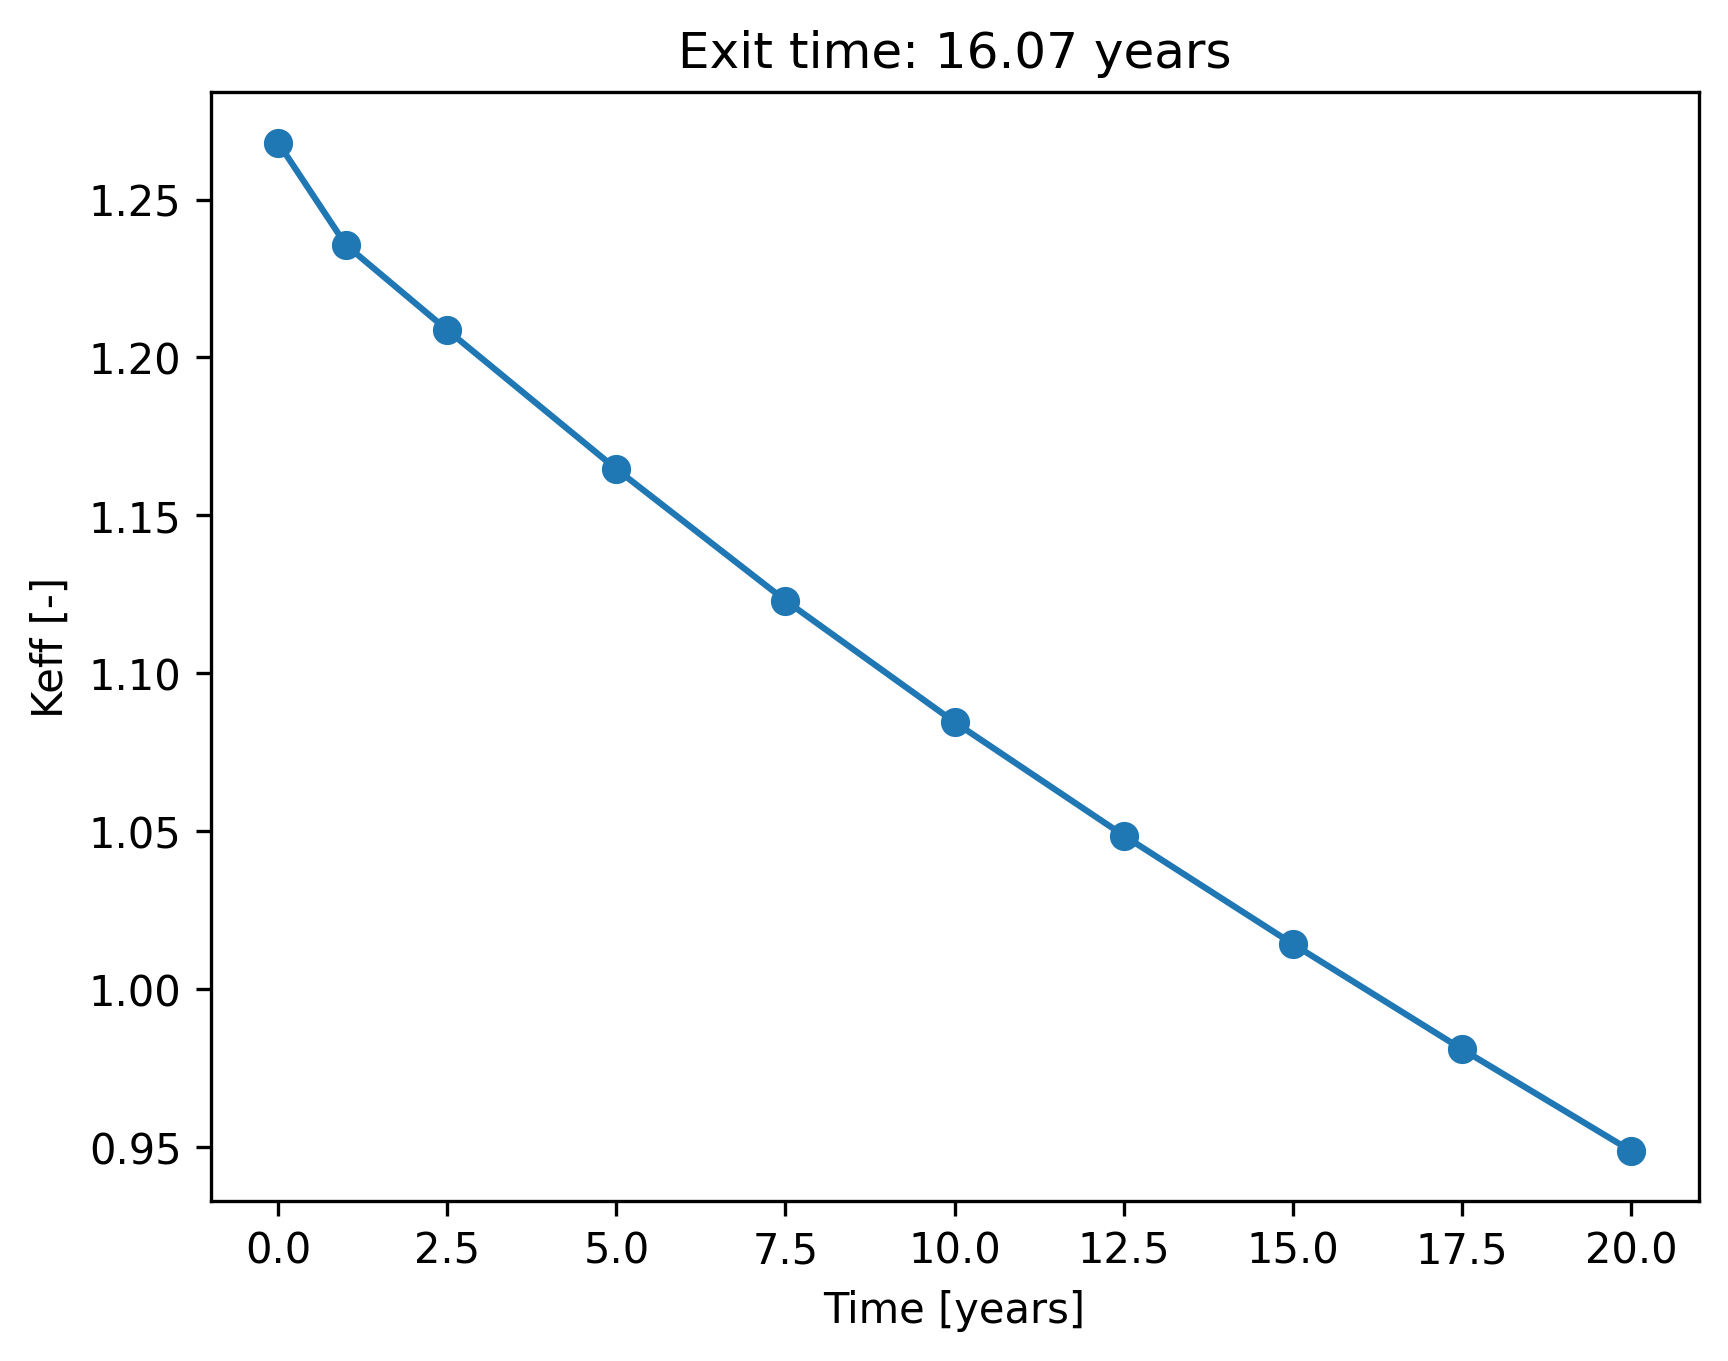
\includegraphics[width=0.55\linewidth]{figures/keff-irrad-time}
  \end{center}
  \caption{$\mu$HTGR $K_{eff}$ time evolution.}
  \label{fig:res-1}
\end{figure}

% heterogenous model results
Figure \ref{fig:res-2} shows the dose rate map at the citadel after a 3-month cool-down.
The region directly above the reactor core shows the largest values, some of them being above 40 mSv/h.
The dose rate in the standard person is 6.48 +/- 1.04 mSv/h.

\begin{figure}[htbp!]
  \begin{center}
    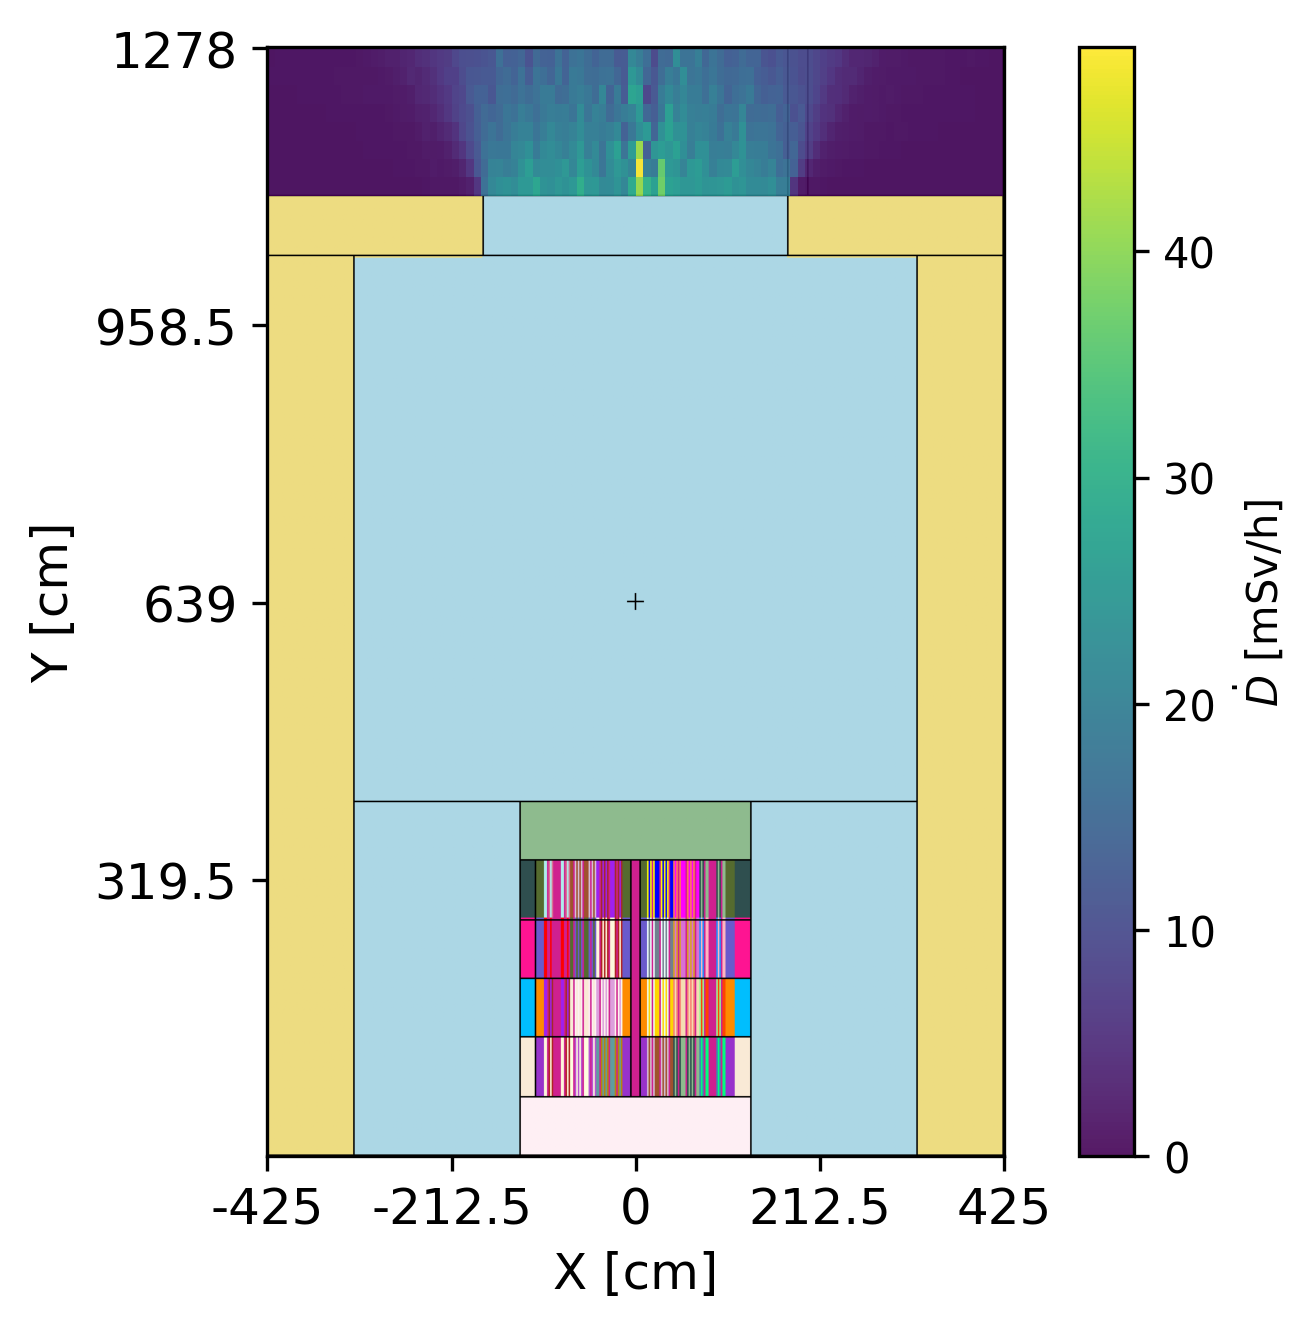
\includegraphics[width=0.60\linewidth]{figures/meshtal4}
  \end{center}
  \caption{Dose rate map at the citadel after 3 month-cool-down.}
  \label{fig:res-2}
\end{figure}

% Discussion
% Title 10, Part 20, of the Code of Federal Regulations (10 CFR Part 20) "Standards for Protection against Radiation".
% https://www.nrc.gov/about-nrc/radiation/health-effects/info.html#dose
The annual total effective dose equivalent for the whole body is 50 mSv for radiation workers.
Although the calculated dose rate is below this limit, other considerations need to be considered, such as exposure time and worker's distance.
These working conditions would allow a radiation worker to perform their tasks for less than 8 hours per year.
Additionally, the calculations consider a vertical distance of 7 m between the top of the core and the worker.
However, while the assemblies are being removed, such a distance will be considerably smaller, and the dose rate will increase accordingly.
For this reason, other decommissioning strategies should be considered to minimize unnecessary exposure.
% Conclusions 10-
Future work should analyze those strategies, adding shielding to the reactor core/assemblies and allowing for a longer cool-down time.


\section{Conclusions}
\label{sec:conclusion}

% Intro
This chapter focuses on the shutdown-dose rate calculations, which are necessary for the determination of suitable \gls*{PIE} strategies for experiment irradiation.
Benefiting from similar workflows, a minimal modification of the workflow allows to obtain both delayed heating and shutdown dose rate.

Motivated by the calculation of shutdown dose rates in experiments, the \gls*{AGR1} experiment sets the path forward for the application of this workflow to \glspl*{HTGR}.
To properly model the AGR-1 experiment, it is insightful to understand the calculation workflow for HTGRs.
% 13- Intro
Additionally, as \gls*{HTGR} technology has distinct features from \glspl*{LWR}, their decommissioning requires new strategies that can be guided by the shutdown dose rate calculations.

% 13- Background
The current available literature on dose rate calculations of HTGRs is scarce, and it focuses on the normal operation regime.
Additionally, previous work on shutdown dose rates of HTGRs lacks the definition of a formal methodology that considers the double heterogeneity of the TRISO fuel.
This thesis introduces a new shutdown dose rate calculation capability for HTGRs that relies on MOAA and the MCNP repeated structures to explicitly model the decay radiation emitted from the TRISO particles.
% 13 - Method
MOAA is responsible for conducting the first two steps of the process, while the third step is conducted by an MCNP photon transport simulation.

% 13- Results
This work introduces a simple exercise to verify the workflow.
For this exercise, one calculation employs the explicit independent definition of each source cell and provides the reference values, while a second calculation utilizes the repeated structures' approach.
% Even though the results for the repeated structures' case show an overestimation of the delayed heating, which is mainly attributed to the problem geometry, the approach seems to yield a reasonable approximation.
The results for the repeated structures' case show that the approach yields a reasonable approximation when the flux spatial variations are considered.

% 13- Results
Finally, this chapter showcases the shutdown dose rate calculation capabilities by presenting two exercises.
These exercises calculate the shutdown dose rate of the AGR-1 TRISO-fueled experiment and a high-temperature gas-cooled microreactor, the $\mu$HTGR.
For the AGR-1 experiment, the results showed that the largest contributor to the dose is the fuel for most decay times.
However, for different decay times, some of the structures produce comparable intensities to the fuel, such as the Hf shroud and the stainless steel structures.
Additionally, the results lead to the recommendation of allowing a decay time of more than one year and the addition of appropriate shielding for conducting the PIE.
For the $\mu$HTGR, the results showed that the proposed decommissioning strategy is feasible but not ideal, as it would lead to very high exposures.
Hence, these results open the door for future studies, which consider the addition of shielding to the reactor core/assemblies and allowing for a longer cool-down time.
